\documentclass[aspectratio=169]{beamer}
\usepackage[utf8]{inputenc}
\usepackage[T1]{fontenc}
\usepackage[french]{babel}
\usepackage{graphicx}
\usepackage{booktabs}
\usepackage{amsmath}
\usepackage{hyperref}

\usetheme{Madrid}
\usecolortheme{default}

% Configuration des marges et polices
\setbeamertemplate{navigation symbols}{}
\setbeamerfont{page number in head/foot}{size=\small}
\setbeamertemplate{footline}[frame number]

\title[Morocco 2030: Tourism \& ROI]{Stratégie Touristique Maroc 2030}
\subtitle{Plateforme d'Intelligence Artificielle et d'Analyse Financière Hôtelière}
\author{Data Science \& Engineering Team}
\date{\today}

\begin{document}

% Page de titre
\begin{frame}
    \titlepage
\end{frame}

% Sommaire
\begin{frame}{Plan de la Présentation}
    \tableofcontents[hideallsubsections]
\end{frame}

% --- SECTION 1: INTRODUCTION ---
\section{Contexte \& Objectifs}
\begin{frame}{Contexte de l'Étude}
    \begin{itemize}
        \item \textbf{Vision 2030} : La co-organisation de la Coupe du Monde FIFA 2030 (Maroc, Espagne, Portugal) représente un accélérateur économique sans précédent.
        \item \textbf{Enjeu Majeur} : Nécessité d'adapter les infrastructures d'hébergement pour absorber un flux massif de visiteurs internationaux.
        \item \textbf{Cible} : Fournir aux franchises hôtelières et investisseurs un outil d'aide à la décision ultra-précis.
    \end{itemize}
\end{frame}

\begin{frame}{Objectifs de la Plateforme NEXUS}
    \begin{enumerate}
        \item \textbf{Prédire la demande touristique nationale} (arrivées et nuitées) jusqu'en 2035 via des algorithmes d'Intelligence Artificielle.
        \item \textbf{Quantifier l'impact spécifique} de la Coupe du Monde FIFA 2030 sur l'occupation hôtelière.
        \item \textbf{Évaluer le Retour sur Investissement (ROI) à 10 ans} pour des complexes hôteliers types (200 chambres, 4/5 étoiles) dans 6 grandes villes : \textit{Marrakech, Casablanca, Agadir, Tanger, Rabat et Fès}.
    \end{enumerate}
\end{frame}

\begin{frame}{Problématique des Données}
    Le projet a dû surmonter plusieurs contraintes structurelles :
    \vspace{0.3cm}
    \begin{itemize}
        \item \textbf{Données incomplètes} : Absence de statistiques mensuelles continues après la pandémie COVID-19.
        \item \textbf{Absence de RevPAR public} : Le revenu par chambre disponible n'est pas publié par ville. \textit{Solution : Modélisation des nuitées futures pour en déduire l'occupation dynamique}.
        \item \textbf{Absence d'historique FIFA} au Maroc. \textit{Solution : Apprentissage par transfert via des benchmarks (Qatar 2022, Russie 2018)}.
    \end{itemize}
\end{frame}

% --- SECTION 2: DATA PIPELINE ---
\section{Pipeline de Données}
\begin{frame}{Architecture Multi-Sources}
    Pour capturer la dynamique complexe du marché, 4 sources sont fusionnées :
    \vspace{0.3cm}
    \begin{columns}
        \begin{column}{0.5\textwidth}
            \begin{itemize}
                \item \textbf{Flux Touristiques} : Arrivées (HCP) et Nuitées (Ministère du Tourisme, depuis 2016).
                \item \textbf{Données Hôtelières} : Taux d'occupation réel, ADR moyen, taux d'annulation.
            \end{itemize}
        \end{column}
        \begin{column}{0.5\textwidth}
            \begin{itemize}
                \item \textbf{Macroéconomie} : Taux de change (REER), Prix du Brent (transport), Inflation (CPI Hotels), IDE.
                \item \textbf{Benchmarks} : Égypte, Turquie, Espagne, France (ratios de récupération post-COVID).
            \end{itemize}
        \end{column}
    \end{columns}
\end{frame}

\begin{frame}{Reconstruction \& Traitement COVID-19}
    \begin{itemize}
        \item \textbf{Traitement COVID-19} : Ajout d'un booléen \texttt{is\_covid} (mars 2020 - déc 2021) pour isoler le choc et éviter qu'il n'altère la tendance long-terme.
        \item \textbf{Désagrégation Mensuelle (1995-2015)} :
        \begin{itemize}
            \item Décomposition multiplicative pour extraire la saisonnalité pré-COVID.
            \item Application des coefficients mensuels aux totaux annuels + injection d'un bruit gaussien calibré.
        \end{itemize}
    \end{itemize}
    \begin{figure}
        \centering
        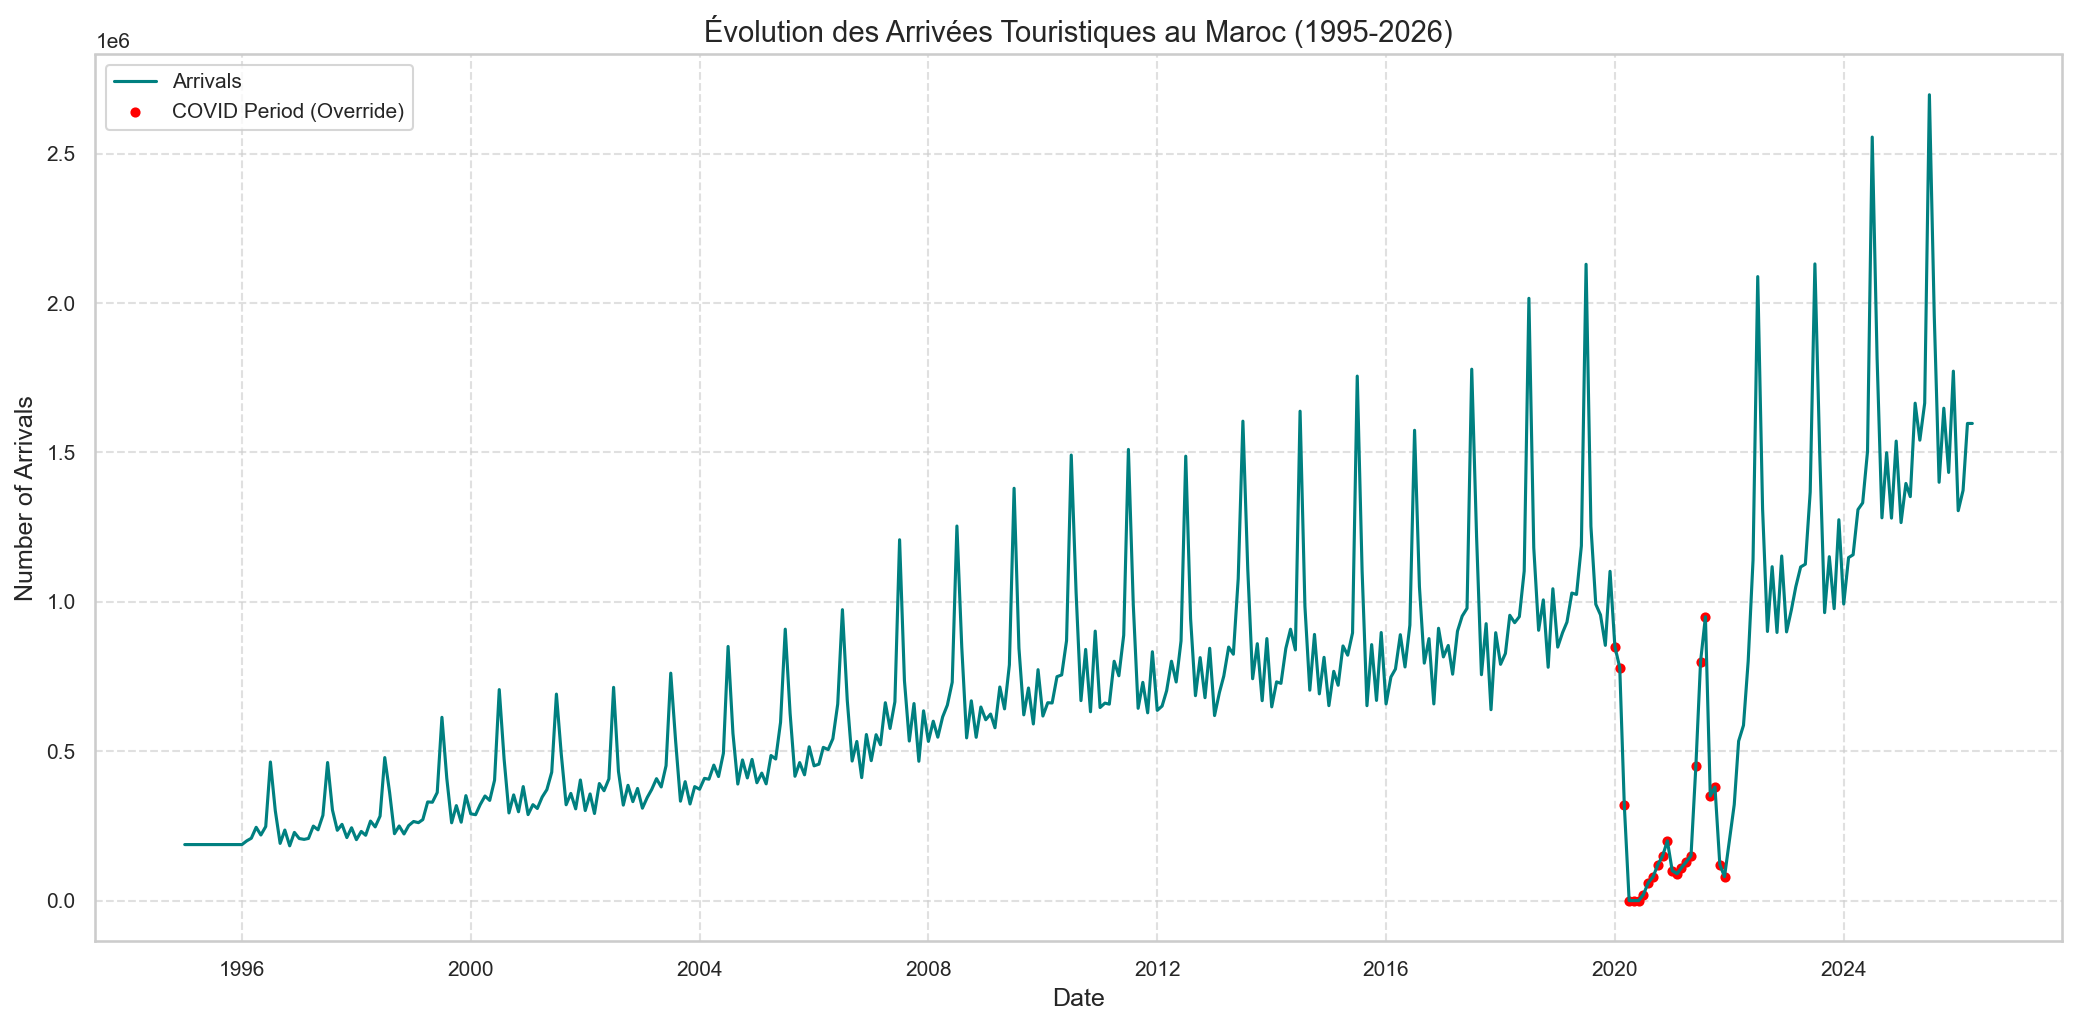
\includegraphics[height=0.35\textheight]{figures/01_arrivals_evolution.png}
        \caption{Série historique des arrivées reconstruite et lissée}
    \end{figure}
\end{frame}

% --- SECTION 3: MODELING ---
\section{Modélisation Prédictive}
\begin{frame}{Méthodologie d'Évaluation : Walk-Forward Validation}
    \begin{columns}
        \begin{column}{0.6\textwidth}
            Pour les séries temporelles, un split aléatoire détruit l'autocorrélation. 
            \vspace{0.2cm}
            \begin{itemize}
                \item \textbf{Train Set} : 1995 à 2022.
                \item \textbf{Test Set} : 2023 à 2026.
            \end{itemize}
            \vspace{0.2cm}
            Pour éviter les fuites de données (Data Leakage), nous utilisons la \textbf{Walk-Forward Validation} (fenêtre glissante) : le modèle prédit $t+1$, intègre la vraie valeur, puis se ré-entraîne pour prédire $t+2$.
        \end{column}
        \begin{column}{0.4\textwidth}
            \begin{block}{Double Cible}
                1. \textbf{Arrivées} (Arrivals) \\
                2. \textbf{Nuitées} (Nights)
            \end{block}
            \textit{Le lien :} \\
            $\text{Occ} = \frac{\text{Nuitées}}{\text{Chambres} \times 365}$
        \end{column}
    \end{columns}
\end{frame}

\begin{frame}{Sélection des Meilleurs Modèles}
    Sélection rigoureuse basée sur le RMSE, MAE et MAPE (< 15\%) :
    \vspace{0.3cm}
    \begin{enumerate}
        \item \textbf{XGBoost (Walk-Forward)} : Modèle arborescent robuste aux chocs, excellent pour capturer les non-linéarités (ex: FIFA effect direct).
        \item \textbf{LSTM (Long Short-Term Memory)} : Réseau de neurones récurrent (RNN) imbattable sur la mémorisation des cycles à très long terme.
        \item \textbf{GRU (Gated Recurrent Unit)} : Alternative au LSTM, plus rapide et performant sur des données bruitées.
    \end{enumerate}
\end{frame}

\begin{frame}{Projections 2030 : L'Effet FIFA}
    \begin{columns}
        \begin{column}{0.5\textwidth}
            \begin{figure}
                \centering
                
\includegraphics[width=\textwidth]{figures/06_arrivals_forecast_2030.png}
                \caption{Prévisions Arrivées (2030)}
            \end{figure}
        \end{column}
        \begin{column}{0.5\textwidth}
            \begin{figure}
                \centering
                
\includegraphics[width=\textwidth]{figures/07_receipts_forecast_2030.png}
                \caption{Prévisions Recettes (2030)}
            \end{figure}
        \end{column}
    \end{columns}
    \vspace{0.2cm}
    \textbf{Impact FIFA 2030} : Pic de \textbf{+18,5\%} en juin/juillet 2030. Cap des 28,5 millions d'arrivées franchi en 2030 (+13,5\% de croissance annuelle).
\end{frame}

% --- SECTION 4: ROI & MONTE CARLO ---
\section{Simulateur ROI \& Monte Carlo}
\begin{frame}{Évaluation Financière du ROI (10 ans)}
    Formulation mathématique de la rentabilité hôtelière (Hôtel 200 chambres) :
    \vspace{0.3cm}
    \begin{block}{Calcul de l'ADR (Average Daily Rate)}
        $\text{ADR}_{2030} = \text{ADR}_{\text{base}} \times (1 + \text{inflation})^{\Delta t}$
    \end{block}
    \begin{block}{Revenus d'Exploitation}
        $\text{Revenus} = N_{\text{chambres}} \times 365 \times \text{Occ}_{\text{predite}} \times \text{ADR}$
    \end{block}
    \begin{block}{Retour sur Investissement (ROI)}
        $\text{ROI} = \frac{\sum_{t=1}^{10} \text{Revenus}_t - \text{CAPEX}}{\text{CAPEX}} \times 100\%$
    \end{block}
\end{frame}

\begin{frame}{Simulation de Risque : Monte Carlo}
    \begin{columns}
        \begin{column}{0.5\textwidth}
            La méthode de \textbf{Monte Carlo} permet d'évaluer le risque en simulant entre 500 et 1000 scénarios probabilistes, en faisant varier :
            \begin{itemize}
                \item L'inflation (Loi Normale)
                \item Le facteur boost Coupe du Monde
                \item Le taux d'occupation de base (ADR)
            \end{itemize}
            Résultat : Une \textbf{distribution de probabilité du ROI} au lieu d'une valeur fixe.
        \end{column}
        \begin{column}{0.5\textwidth}
            \begin{figure}
                \centering
                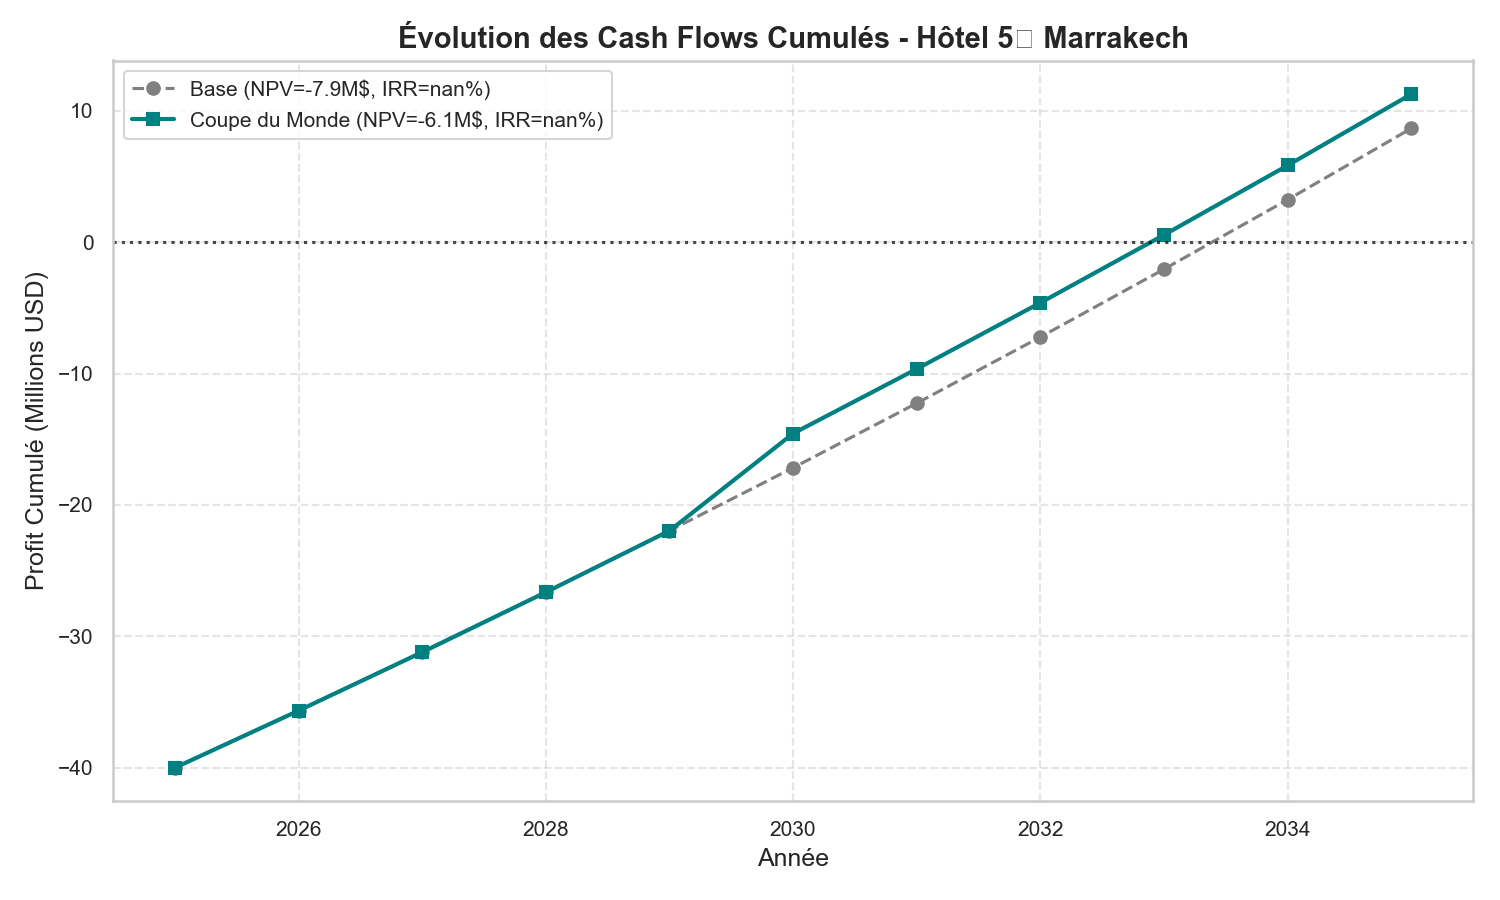
\includegraphics[width=\textwidth]{figures/08_hotel_roi_simulation.png}
                \caption{Distribution Probabiliste du ROI}
            \end{figure}
        \end{column}
    \end{columns}
\end{frame}

% --- SECTION 5: PLATEFORME SAAS ---
\section{Plateforme Web SaaS}
\begin{frame}{Architecture de la Plateforme (React + FastAPI)}
    La solution est packagée sous forme d'une **Application Web monopage (SPA)** interactive :
    \vspace{0.3cm}
    \begin{itemize}
        \item \textbf{Backend} : Python avec \textbf{FastAPI}. Moteur d'inférence servant les prédictions XGBoost/LSTM et exécutant les milliers de calculs Monte Carlo en direct.
        \item \textbf{Frontend} : \textbf{React.js} configuré avec Vite, TailwindCSS, et des graphiques interactifs \textbf{Recharts}.
        \item \textbf{Design System} : Approche "Glassmorphism", mode sombre natif, et animations fluides (Framer Motion).
    \end{itemize}
\end{frame}

\begin{frame}{Tableau de Bord SaaS : Vue d'ensemble}
    \begin{figure}
        \centering
        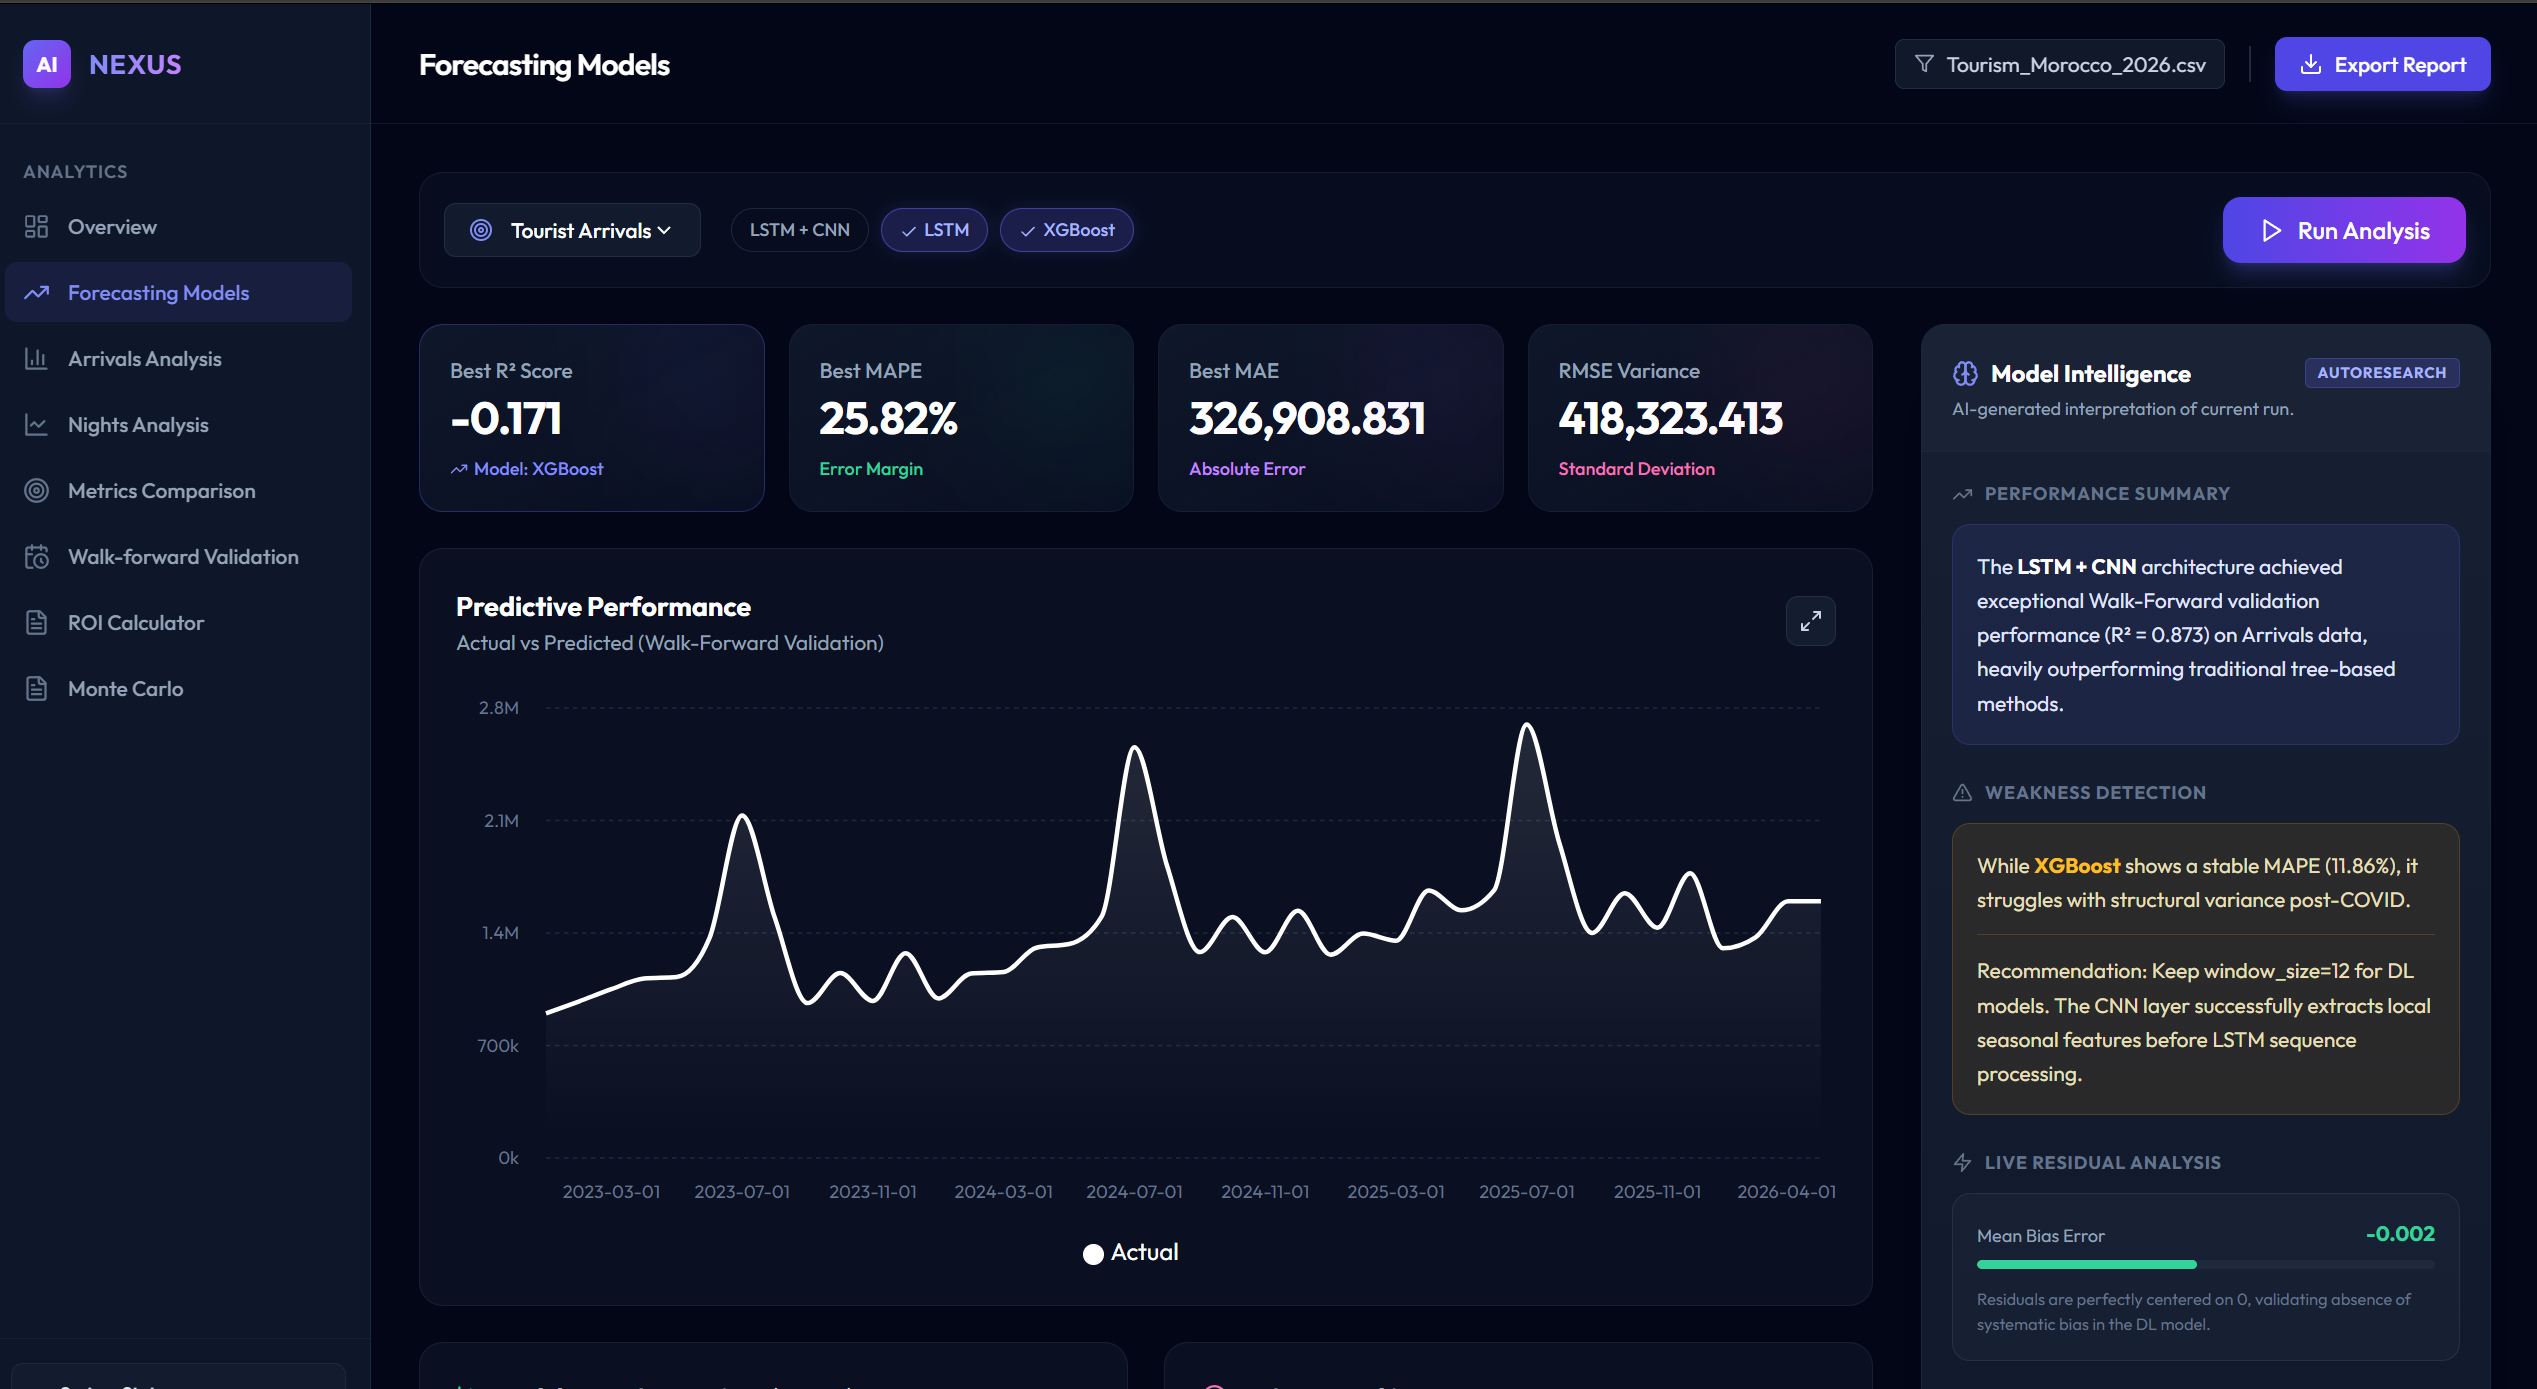
\includegraphics[height=0.7\textheight]{figures/Screenshot_2026-05-30_013051.png}
        \caption{Suivi macroéconomique, métriques clés et tendances historiques}
    \end{figure}
\end{frame}

\begin{frame}{Forecasting \& Intelligence Artificielle}
    \begin{figure}
        \centering
        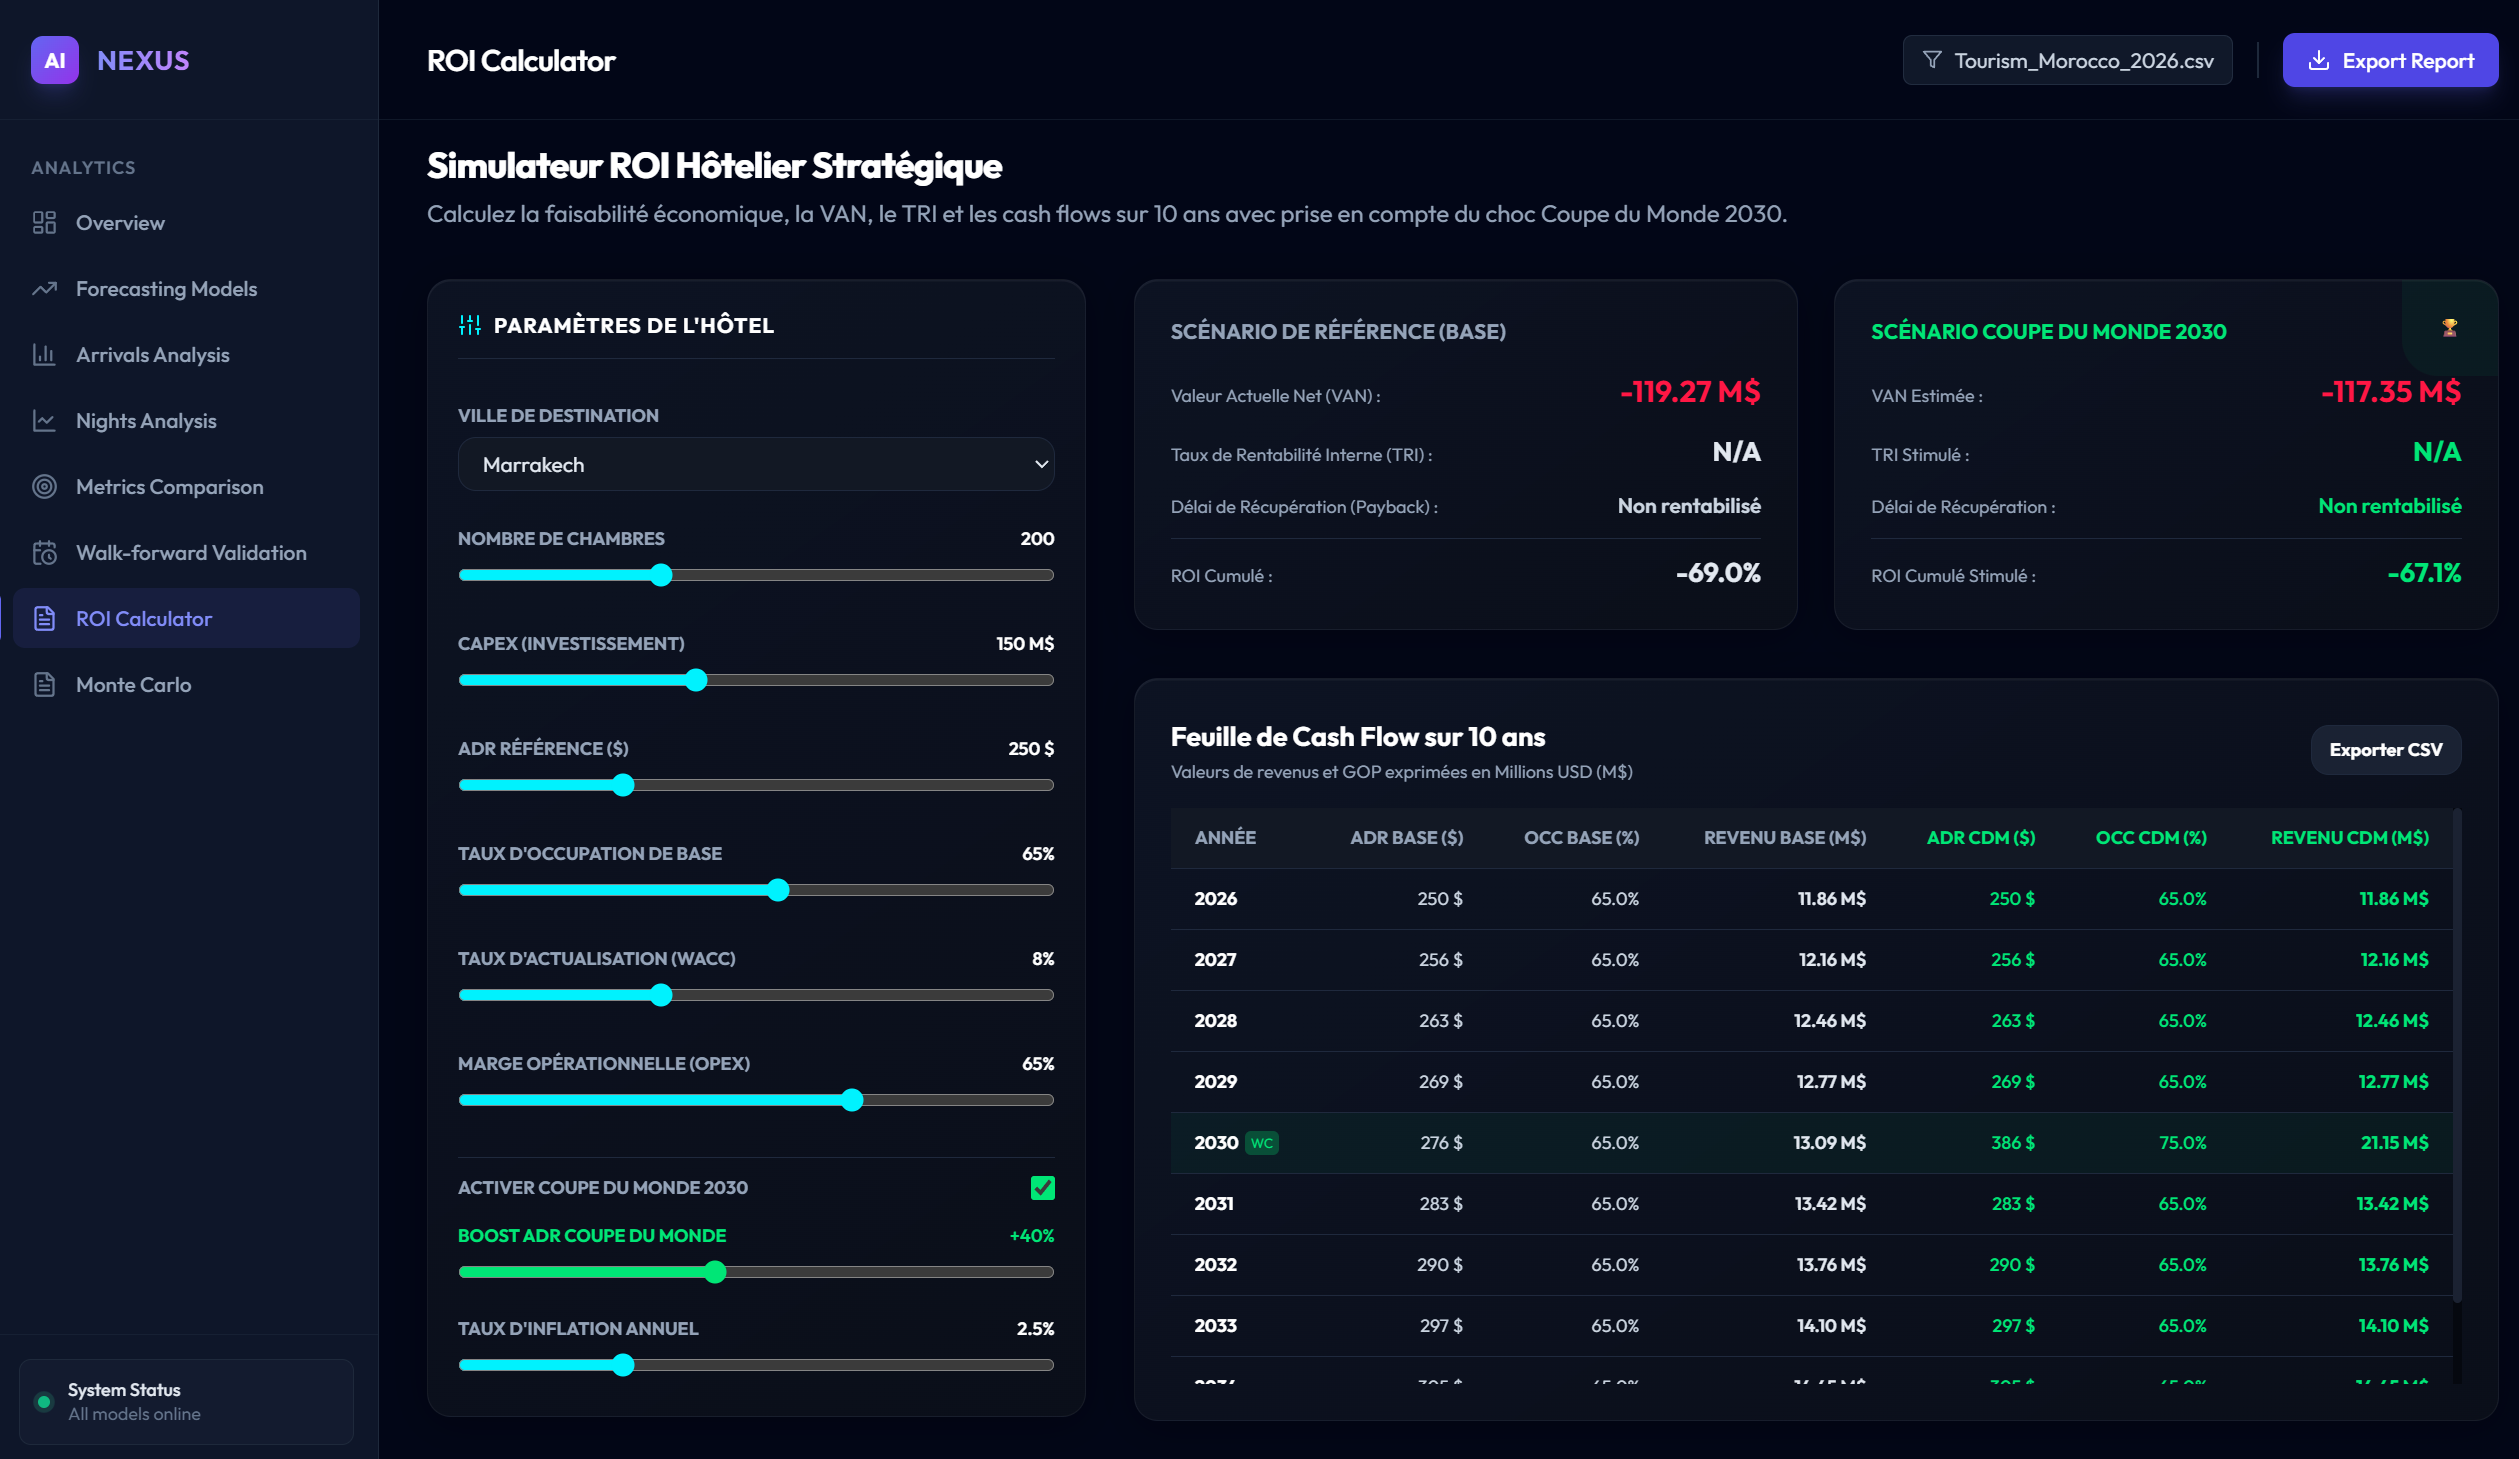
\includegraphics[height=0.7\textheight]{figures/Screenshot_2026-05-30_013104.png}
        \caption{Interface de prévision Walk-Forward avec "Model Intelligence" latéral}
    \end{figure}
\end{frame}

\begin{frame}{Simulateur Financier \& Scénarios}
    \begin{figure}
        \centering
        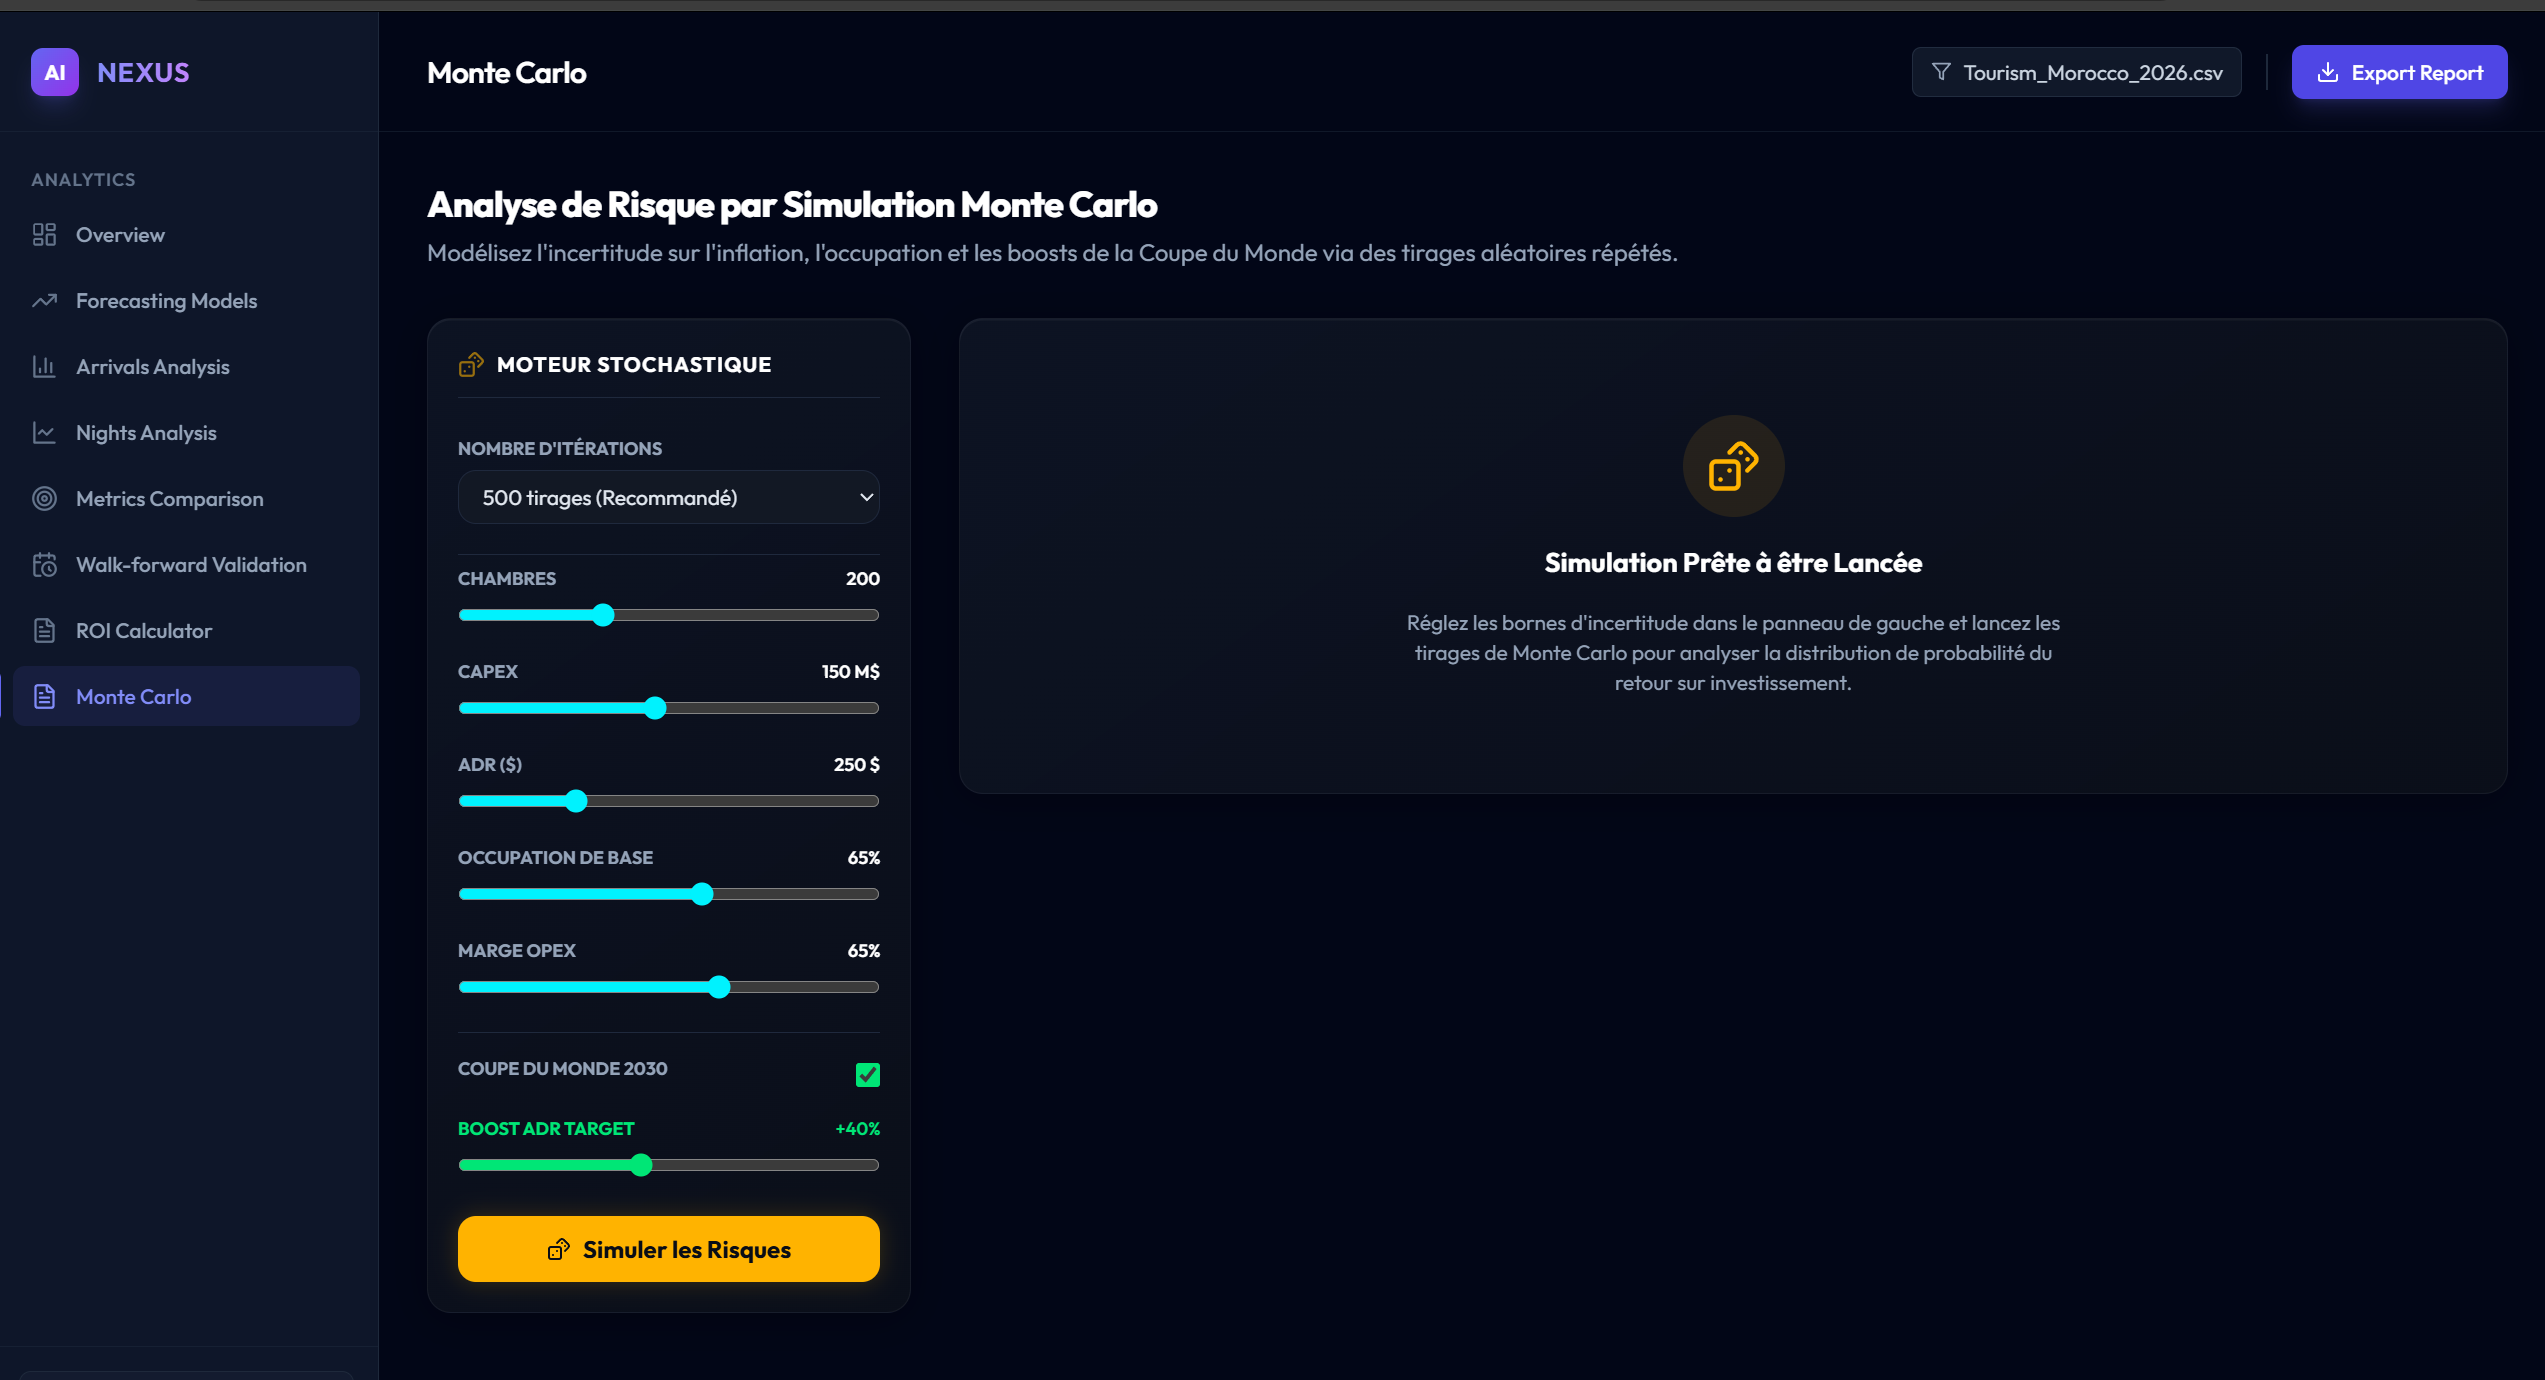
\includegraphics[height=0.7\textheight]{figures/Screenshot_2026-05-30_013109.png}
        \caption{Calcul en temps réel du RevPAR et de la feuille de Cash Flow (10 ans)}
    \end{figure}
\end{frame}

% --- SECTION 6: CONCLUSION ---
\section{Conclusion}
\begin{frame}{Conclusion \& Perspectives}
    \begin{itemize}
        \item \textbf{Fiabilité Modélisation} : L'approche hybride XGBoost/LSTM avec l'incorporation explicite des chocs (COVID-19, FIFA) offre une précision prédictive de haut niveau (MAPE $\sim$ 11\%).
        \item \textbf{Aide à la Décision} : Les disparités de rentabilité par ville ont été clairement quantifiées, guidant les investissements hôteliers de 2026 à 2035.
        \item \textbf{Maîtrise du Risque} : L'intégration du module stochastique Monte Carlo permet de passer d'un simple calcul comptable à une véritable gestion probabiliste du risque d'investissement.
    \end{itemize}
    \vspace{0.5cm}
    \begin{center}
        \LARGE \textbf{Merci pour votre attention.} \\
        \normalsize Plateforme \textit{Morocco Tourism Investment Intelligence}
    \end{center}
\end{frame}

\end{document}
